%%%%%%%%%%%%%%%%%%%%%%%%%%%%%%%%%%%%%%%%%%%%%%%%%%%%%%%%%%%%%%%%%%%%%%%%
%                                                                      %
% LaTeX, FIIW thesis template                                          %
% 28/11/2014 v1.2                                                      %
%                                                                      %
%%%%%%%%%%%%%%%%%%%%%%%%%%%%%%%%%%%%%%%%%%%%%%%%%%%%%%%%%%%%%%%%%%%%%%%%
\documentclass[11pt,a4paper]{report}
% Indien je je thesis recto-verso wil afdrukken gebruik je onderstaande opties i.p.v. bovenstaande
%\documentclass[11pt,a4paper,twoside,openright]{report}

\usepackage[a4paper,left=3.5cm, right=2.5cm, top=3.5cm, bottom=3.5cm]{geometry}
\usepackage[english]{babel}
\usepackage{titlesec}

\setcounter{secnumdepth}{100}

\titleclass{\subsubsubsection}{straight}[\subsection]

\newcounter{subsubsubsection}[subsubsection]
\renewcommand\thesubsubsubsection{\thesubsubsection.\arabic{subsubsubsection}}
\renewcommand\theparagraph{\thesubsubsubsection.\arabic{paragraph}} % optional; useful if paragraphs are to be numbered

\titleformat{\subsubsubsection}
  {\normalfont\normalsize\bfseries}{\thesubsubsubsection}{1em}{}
\titlespacing*{\subsubsubsection}
{0pt}{3.25ex plus 1ex minus .2ex}{1.5ex plus .2ex}

\makeatletter
\renewcommand\paragraph{\@startsection{paragraph}{5}{\z@}%
  {3.25ex \@plus1ex \@minus.2ex}%
  {-1em}%
  {\normalfont\normalsize\bfseries}}
\renewcommand\subparagraph{\@startsection{subparagraph}{6}{\parindent}%
  {3.25ex \@plus1ex \@minus .2ex}%
  {-1em}%
  {\normalfont\normalsize\bfseries}}
\def\toclevel@subsubsubsection{4}
\def\toclevel@paragraph{5}
\def\toclevel@paragraph{6}
\def\l@subsubsubsection{\@dottedtocline{4}{7em}{4em}}
\def\l@paragraph{\@dottedtocline{5}{10em}{5em}}
\def\l@subparagraph{\@dottedtocline{6}{14em}{6em}}
\makeatother

\usepackage{graphicx}
%\usepackage[latin1]{inputenc}           % om niet ascii karakters rechtstreeks te kunnen inputten
\usepackage[utf8]{inputenc}            % commentarieer deze regel uit als je utf8 encoded files gebruikt in plaats van latin1
\usepackage[numbers]{natbib}
\usepackage{listings}             		% voor het weergeven van broncode
\usepackage{verbatim}					% weergeven van code, commando's, ...
\usepackage[hidelinks]{hyperref}		% maak PDF van de thesis navigeerbaar without boxes
%\usepackage{hyperref}					% maak PDF van de thesis navigeerbaar
\usepackage{url}						% URL's invoegen in tekst met behulp van \url{http://}
\usepackage[small,bf,hang]{caption}     % om de captions wat te verbeteren
\usepackage[final]{pdfpages}            % gebruikt voor het invoegen van het artikel in pdf-formaat
\usepackage{pslatex}					% andere lettertype's dan de standaard types
\usepackage{lipsum}
\usepackage{sectsty}					% aanpassen van de fonts van sections en chapters
%\usepackage[nottoc,numbib]{tocbibind}	% Bibliography mee in de ToC
\usepackage{tikz}
\usepackage{xcolor}
\usepackage{standalone}
\usepackage{enumitem}
\usepackage{multirow}
\usepackage{chngpage}
\setlist{nosep}
%\usetikzlibrary{external}

\allsectionsfont{\sffamily}
\chapterfont{\raggedleft\sffamily}

\usepackage{float}                      % De optie H voor de plaatsing van figuren op de plaats waar je ze invoegt. bvb. \begin{figure}[H]
%\usepackage{longtable}					% tabellen die over meerdere pagina's gespreid worden
%\usepackage[times]{quotchap}           % indien je fancy hoofdstuktitels wil
%\usepackage[none]{hyphenat}
%\usepackage{latexsym}
\usepackage{amsmath}
\usepackage{amssymb}

% MFA: zet zoekpad voor figure
\usepackage{subcaption}
\graphicspath{{fig/}}

\usepackage{fiiw_eng}

%door onderstaande regels in commentaar te zetten, of op false, kan je pagina's weglaten
%bijvoorbeeld het weglaten van een voorwoord, lijst met symbolen, ...
%%%%%%%%%%%%%%%%%%%%%%%%%%%%%%%%%%%%%%%%%%%%%%%%%%%%%%%%%%%%%%%%%%%%%%%%%%%%%%%%%%%%%%%%
%voorwoord toevoegen?
\acknowledgementspagetrue
\acknowledgements{voorwoord}			%.tex file met daarin het voorwoord

%samenvatting toevoegen
\summarypagetrue
\summary{samenvatting}					%.tex met daarin de samenvatting

%abstract toevoegen?
\abstractpagetrue
\abstracts{abstract}					%.tex file met daarin het abstract
%lijst van figuren toevoegen?
\listoffigurespagetrue
%lijst van tabellen toevoegen?
% \listoftablespagetrue
%lijst van symbolen toevoegen?
%\listofsymbolspagetrue
\listofsymbols{symbolen}				%.tex file met daarin de lijst van symbolen



%informatie over het eindwerk, de promotor, ...
%%%%%%%%%%%%%%%%%%%%%%%%%%%%%%%%%%%%%%%%%%%%%%%
\opleiding{E-ICT}
\afdeling{Software Engineer - option ICT}

\campus{denayereng} %denayer,denayereng,geel,geeleng,gent,ghenteng,groept,groupteng,brugge,brugeseng

\title{Counting shells}
\subtitle{Are current neural networks performant enough to count various types of shells in an uncontrolled environment?}
% \author{naam student}
\forenameA{ }
\surnameA{ }

% l
\forenameB{Tijs}
\surnameB{Van Kampen}

\academicyear{2022 - 2023}

\promotorA[Promotor]{Prof. Dr. Ir. Toon Goedemé}
\promotorB[Co-Promotor]{Dr. Ing. Tanguy Ophoff}

\begin{document}
%\selectlanguage{dutch} %due to incompatible syntax with the English style library and the extended features of the dutch library, I'll be modifying the dutch library to be English
\selectlanguage{english} % For the English version
\preface

%%%%%%%%%%%%%%%%%%%%%%%%%%%%%%%%%%%%%%%%%%%%%%%%%%%%%%%%%%%%%%%%%%% 
%                                                                 %
%                            CHAPTER                              %
%                                                                 %
%%%%%%%%%%%%%%%%%%%%%%%%%%%%%%%%%%%%%%%%%%%%%%%%%%%%%%%%%%%%%%%%%%% 

\chapter{Introduction}

Once per year, nearly a thousand volunteers travel to the Belgian coast to collect and categorize the shells that wash up on the beach. This data is collected by the Flemish Institute For The Sea (VLIZ) to study populations of marine mollusks and the impact of their environment (climate change, fishing, etc) on the population. The volunteers participating in this study are mostly enthusiasts, but also scientists and families with children. To ensure the quality of the data, most volunteers participate in a workshop prior to the activity. The counting of the shells is done by walking along the beach and logging every individual shell that is found. This is a very time-consuming process, and the volunteers are often not very experienced in counting, resulting in mistakes with all but the most common shells. When a volunteer finds a shell that they are not familiar with, they can contact a helpdesk to help them. The flowchart of the current process can be found in Figure \ref{fig:1_current_scenario}. 

\begin{figure}[h]
	\centering
	\includegraphics[width=1\textwidth]{chapter1/current_scenario}
	\captionsetup{belowskip=-\baselineskip}
	\caption{The current process of collecting data.}
	\label{fig:1_current_scenario}
	\setlength\belowcaptionskip{\baselineskip}
	\caption*{Marked blue is the volunteer's actions, and marked red are the parts that involve experts.}
\end{figure}

The fact that the project relies on volunteers to do most of the legwork, combined with experts having to man the checkpoints and the helpdesk, makes the project unscalable beyond having a single dedicated day each year. With over 5 million people
%https://www.kustportaal.be/nl/toerisme-en-recreatie#:~:text=De%20Belgische%20kust%20is%20de,in%20totaal%2027.723.420%20overnachtingen.
visiting the Belgian coast every year\cite{Kustportaal}, there is a lot of potential data to collect. To use this source of data, the process would have to be simplified and accessible to anyone visiting the beach at any time.

In this thesis, we will attempt to simplify the process of data collection so that it can be done by anyone, anywhere, at any time. We will do this with a counting network so that shells can be recognized in an image and counted automatically. This is already done on a smaller scale by VLIZ with Obsidentify, a mobile app and website where users can submit pictures of a single shell and get a result of what kind of shell it is. This is a useful tool, but taking a close-up picture of every single shell is again a very time-consuming process. 

As no dataset exists with large quantities of annotated pictures of beaches, we will have to work with a dataset of limited size to evaluate or train the neural network. After the successful completion of this thesis, the new ideal scenario for collecting data can be found in Figure \ref{fig:1_ideal_scenario}. Compared to the current process, found in Figure \ref{fig:1_current_scenario}, this new process nearly eliminates the experts' involvement and thus makes the process scalable.

\begin{figure}[h]
	\centering
	\includegraphics[width=0.8\textwidth]{chapter1/ideal_scenario}
	\caption{The new process of collecting data.}
	\label{fig:1_ideal_scenario}
\end{figure}

We will be testing if current counting networks are performant enough to recognize shells in beach images. We will do this by first introducing our dataset on which we will evaluate various methods. We will then discuss the state of the art in the field of object detection and counting, with a focus on few-shot learning. We then discuss how we will implement the models we studied. Next, the results and the limitations of the models are discussed. Finally, we will discuss future work that can be done to improve the model.
\chapter{Dataset}
In this chapter, we will describe the few-shot shell dataset we are introducing.

Many datasets exist for object detection. These can be split into two categories, general datasets and specialized datasets. General datasets are datasets that contain a wide variety of object classes, such as COCO \cite{COCO}, OpenImages \cite{OpenImages}, and ImageNet \cite{ImageNet}. Specialized datasets are datasets that contain a specific category of objects like Oxford Pets \cite{OxfordPets} and Gun Detection \cite{Gundetection}. The general datasets are often used to pre-train a model, while the specialized datasets are used to fine-tune the model to a specific task.

However, no such specialized object detection dataset exists for seashells. Getting a representative dataset of all or most types of shells that could be found in large quantities would be a very time-intensive task. As such we purposefully limit the size of the dataset, so that we can evaluate the performance on a small dataset. 

\section{Images}
The images were taken with a cellphone camera on the Belgian coast near Knokke-Heist. Each image has a size of 6144x8192px. The images are mostly sparse, with 1 to 3 shells per image. The dataset does however also contain a limited amount of denser images. An overview of the density can be found in Figure \ref{fig:annotations_per_img}. 

\begin{figure}[H]
    \centering
    \includegraphics[width=0.8\textwidth]{chapter3/annotations_per_img.png}
    \caption{Overview of the annotations per image in the shell dataset.}
    \label{fig:annotations_per_img}
\end{figure}

\section{Annotations}
The images are annotated in Pascal VOC \cite{PASCALVOC} style. As such the annotations are saved in separate XML files, one for each image. In total 96 images are annotated with 614 annotations in total over 9 classes. As shown in Figure \ref{fig:annotations_per_class}% and Table \ref{tab:shell_annotations}
, the annotations are not evenly distributed over the classes. Some examples of the annotated images can be found in Figure \ref{tab:shell_examples}.


\begin{center}
    \begin{figure}[H]
        \makebox[\textwidth]{\includegraphics[width=0.9\paperwidth]{chapter3/annotations_per_class.png}}
        \caption{Overview of the annotations per class in the shell dataset.}
        \label{fig:annotations_per_class}
    \end{figure}
\end{center}



% \begin{table}[H]
%     \centering
%     \captionsetup{justification=centering}
%     \begin{tabular}{|l|l|}
%     \hline
%     \textbf{Shell type} & \textbf{Number of annotations} \\ \hline
%     Mussel              & 268                            \\ \hline
%     Thick trough shell  & 91                             \\ \hline
%     Cockle              & 89                             \\ \hline
%     Baltic tellin       & 69                             \\ \hline
%     Cut trough shell    & 36                             \\ \hline
%     Banded wedge shell  & 32                             \\ \hline
%     Elliptical trough shell & 18                         \\ \hline
%     Oyster              & 9                              \\ \hline
%     Jackknife clam      & 2                              \\ \hline
%     \end{tabular}
%     \caption{Overview of the annotations per class in the shell dataset.}
%     \label{tab:shell_annotations}
% \end{table}


\section{Limitations}
The dataset is limited in a few ways. In this section, we will discuss these limitations and their impact on our work.

\subsection*{Number of classes and size}

At the last shell-counting day a total of 51 types of shells were found in Belgium, with 66 types of shells being found when looking at all participating countries (Belgium, France, The Netherlands). However, only 8 types of shells are present in the dataset. This is due to the limited variety of shells that were found on the day the dataset was collected. Some shells are more difficult to find or are more rare than others, thus it would be difficult to collect a large number of images of these shells even if more images were collected. Realistically we would either have to put in a lot more time and effort to include sufficient shells of every type or find an alternative that uses less data to process our images. The practical results of our work will be limited to the shells that are present in the dataset, but still give a good indication as to what we can expect from it when applied to other shells.

The dataset consists of only 96 annotated images. This is an extremely small dataset, especially for object detection. Though it would be possible to collect and annotate more images, this would be a time-consuming task. Furthermore, the dataset is large enough to indicate the performance of the model as mentioned above.

\subsection*{Diversity}

The dataset is also limited in diversity, as all images were taken on the same day, at the same location, and with the same camera. This means that the dataset is not representative of the full range of conditions that the model would have to work in.


\begin{figure}[H]
    \centering
    \captionsetup{justification=centering}
    \includegraphics[width=0.3\textwidth]{chapter3/shell_examples/1.jpg} 
    \includegraphics[width=0.3\textwidth]{chapter3/shell_examples/2.jpg} 
    \includegraphics[width=0.3\textwidth]{chapter3/shell_examples/3.jpg}
    \includegraphics[width=0.3\textwidth]{chapter3/shell_examples/4.jpg} 
    \includegraphics[width=0.3\textwidth]{chapter3/shell_examples/5.jpg} 
    \includegraphics[width=0.3\textwidth]{chapter3/shell_examples/6.jpg}
    \includegraphics[width=0.3\textwidth]{chapter3/shell_examples/7.jpg}
    \includegraphics[width=0.3\textwidth]{chapter3/shell_examples/8.jpg}
    \includegraphics[width=0.3\textwidth]{chapter3/shell_examples/9.jpg}
    \caption{Examples of images in the shell dataset.}
    \label{tab:shell_examples}
\end{figure}
%%%%%%%%%%%%%%%%%%%%%%%%%%%%%%%%%%%%%%%%%%%%%%%%%%%%%%%%%%%%%%%%%%% 
%                                                                 %
%                            CHAPTER                              %
%                                                                 %
%%%%%%%%%%%%%%%%%%%%%%%%%%%%%%%%%%%%%%%%%%%%%%%%%%%%%%%%%%%%%%%%%%% 

\chapter{Literature Review}
In this chapter, we will review the state of the art in the field of object counting. We will study the techniques commonly used for counting and go in more depth about the topic of few-shot object detection and why it should be applied to our problem. Finally, we will discuss the metrics used to evaluate the performance of the models.

\section{Crowd Counting}
Counting networks are an established concept in machine learning as numerous papers tackle the issue of counting humans, cars, animals or cells. What those have in common is that they only encompass a small set of possible categories to count and that, as they have a large real-life use, large annotated datasets exist like ShanghaiTech \cite{Shanghaitech} and COWC \cite{COWC}. The problem we are trying to solve is a bit different, as we want to count a large set of objects and yet we don't have a large dataset to train on.

The methodology behind heuristic counting networks is divided into three kinds of methods \cite{s22145286}. The first applies a detection method to the image and then counts the number of detected objects. Many different detection methods can be used, from looking for characteristic features to matching the shape of the objects. The second takes a more global approach by first extracting features, textures, gradients and other information from the image as a whole and then using those to count the objects. The third method is not used on static images but on video. It assumes that the objects are moving in clusters and uses that to predict the movement of the objects and improve detection.

Out of those three methods, the third one is not applicable to our problem as we are trying to detect static objects in a still image.
Both the first and second methods are applicable to our problem, however, both have the problem of requiring a large dataset to train on. We will have to use a method that doesn't require a large dataset, which is where few-shot learning comes in. In the domain of few-shot learning the first method, object detection, is the most common. In the next section, we will go more in-depth about few-shot object detection.

%https://www.mdpi.com/1424-8220/22/14/5286

%https://openaccess.thecvf.com/content/CVPR2022W/L3D-IVU/papers/Ranjan_Vicinal_Counting_Networks_CVPRW_2022_paper.pdf

\section{Object detection}
The history of techniques used for object detection can be split into two parts: traditional methods and deep learning-based methods. Before 2012 the traditional methods were the most common, as hardware was not yet powerful enough to train deep learning models. After 2012, with hardware becoming more powerful, deep learning-based methods became the go-to for more complex problems. The deep learning-based methods can be split into two categories: single-stage and two-stage methods. Two-stage methods split the problem into two stages, first detecting the objects and then classifying them and are thus more accurate but slower than single-stage detectors. In this section, we will go over the history and some of the major milestones in the two-stage detector branch of deep learning as for our problem accuracy is the highest priority.

\subsection{R-CNN \cite{rcnn}}
R-CCN, shown in Fig \ref{fig:2_rcnn}, was the first two-stage deep learning method. It obtains region proposals using a method to obtain category-independent region proposals, like selective search \cite{selectivesearch} and then classifies those regions using a convolutional neural network (CNN). While it obtained a large improvement over the state of the art (SOTA), it was quite slow as with each image it had to run the CNN on 2000 regions to extract features. Many of those 2000 would be redundant as they overlap.

\begin{figure}[H]
	\centering
	\includegraphics[width=1\textwidth]{chapter2/rcnn}
	\caption{\label{fig:2_rcnn} RCNN architecture. Image from \citet{rcnn}.}
\end{figure}

\subsection{SPPNet \cite{sppnet}}
SPPNet, shown in Fig \ref{fig:2_sppnet}, takes a different approach compared to R-CNN. Conventional CNN-based methods are limited by the fact that the fully connected layers at the end of the network require a fixed input size. This means that the input image has to be resized to a fixed size for each region, which leads to loss of information and/or bad representation, this can be seen in Fig \ref{fig:2_rcnn}. SPPNet solves this problem by adding a spatial pyramid pooling layer (SPP) after the last convolutional layer, a comparison with conventional CCNs can be found in Fig \ref{fig:2_sppnetvscnn}. Convolutional layers can take any size as input, this is then pooled to the fixed size required for the fully connected layers by the SPP layer. As the convolutional layers are only run once per image, this greatly improves the speed of the network, reaching 20-100x speedup compared to R-CNN. The SPP layer consists of parallel max-pooling layers with differing amounts of pooling regions, which are then concatenated to form a fixed-length representation, as shown in Fig \ref{fig:2_sppnet}.

\begin{figure}[H]
	\centering
	\includegraphics[width=1\textwidth]{chapter2/SPP.png}
	\caption{\label{fig:2_sppnet} SPPNet architecture. Image from \citet{sppnet}.}
\end{figure}

\begin{figure}[H]
	\centering
	\includegraphics[width=1\textwidth]{chapter2/SPPvsCNN.png}
	\caption{\label{fig:2_sppnetvscnn} Conventional CNN vs SPPNet. Image from \citet{sppnet}.}
\end{figure}

\subsection{Fast R-CNN \cite{fastrcnn}}
Fast R-CNN, shown in Fig \ref{fig:2_fastrcnn}, combines the region proposals of R-CNN with the method of SPPNet. It runs the CNN on the whole image and then applies max pooling for each region proposal, they call this region of interest pooling (RoI pooling). The RoI layer is a special case of the SPP layer, the case where the number of pooling regions is one. As the time-consuming CNN is only run once per image, the training and inference time is greatly improved, while the RoI pooling layer increases the accuracy of the network.

\begin{figure}[H]
	\centering
	\includegraphics[width=1\textwidth]{chapter2/fastrcnn.png}
	\caption{\label{fig:2_fastrcnn} Fast R-CNN architecture. Image from \citet{fastrcnn}.}
\end{figure}

\subsection{Faster R-CNN \cite{fasterrcnn}}
Faster R-CNN, shown in Fig \ref{fig:2_fasterrcnn}, improves on Fast R-CNN by replacing the region proposal method with a region proposal network (RPN). The RPN is a fully convolutional network that takes the feature map from the CNN and outputs a set of rectangular object proposals, each with an objectness score. The RPN is trained end-to-end with the rest of the network, which allows the network to learn the region proposal method that works best for the task at hand. This greatly improves the speed of the network, as the RPN is much faster than the region proposal method used in Fast R-CNN.

\begin{figure}[H]
	\centering
	\includegraphics[width=0.6\textwidth]{chapter2/fasterrcnn.png}
	\caption{\label{fig:2_fasterrcnn} Faster R-CNN architecture. Image from \citet{fasterrcnn}.}
\end{figure}

\subsection{Vision Transformers \cite{vit}}
In recent years, the availability of more data has led to the development of architectures that were not previously possible. One example is the transformer architecture \cite{transformers}, originally designed for natural language processing (NLP) tasks, but now also used in computer vision by \citet{vit} who call their approach Vision Transformers (ViT). ViT applies the standard transformer architecture to images with minimal changes and therefore shares most characteristics with transformers. Transformers perform best when trained on large amounts of data. ViT is pre-trained on either the ImageNet-21k \cite{ImageNet} dataset or the JFT-300M dataset and then fine-tuned for various benchmarks, where it exceeds the CNN-based state-of-the-art. 

As ViT uses transformers, it is important to understand how they work. Its main feature is that it foregoes all convolutional layers for attention layers and fully connected layers. The attention layer is a layer of functions that take a set of queries, keys, and values and return a weighted sum of the values. The weights for this sum are calculated by taking the dot product of the query and key vectors and then applying a softmax function. With multi-head attention multiple attention layers run in parallel, each with different (learned) projections of the queries, keys, and values. The output of these sublayers is then concatenated and linearly projected to the desired output size. The (multi-head) attention layer is illustrated in Figure \ref{fig:2_attention}.

The ViT architecture is illustrated in Figure \ref{fig:2_vit}. The model starts by dividing the image into a fixed number of patches, which are linearly projected into a 1D vector. To account for the position of each patch, a position embedding is added to the input.

\begin{figure}[H]
	\centering
	\includegraphics[width=0.8\textwidth]{chapter2/attention.png}
	\caption{\label{fig:2_attention} Attention layer. Image from \citet{transformers}.}
\end{figure}

\begin{figure}[H]
	\centering
	\includegraphics[width=0.8\textwidth]{chapter2/vit.png}
	\caption{\label{fig:2_vit} ViT architecture. Image from \citet{vit}.}
\end{figure}




\section{Few-shot object detection}
%https://arxiv.org/abs/2112.11699
%https://ieeexplore-ieee-org.kuleuven.e-bronnen.be/stamp/stamp.jsp?tp=&arnumber=1597116
%add a reference to the first paper that did it
Few-shot object detection is a technique that has been gaining popularity in the last few years, but interest in training a neural network to classify without a big annotated dataset appeared as early as 2008 with zero-shot learning in \citet{aaai08-132}. It allows us to train a model with few annotated images, which is useful in scenarios where it is not possible to get a large annotated dataset. Few-shot attempts to mirror the way humans learn. During our life, we come across many new objects and we can recognize them even though we only saw them a few times. We do this by building on our knowledge of other objects and using that to recognize the new object \cite{biederman1987recognition}. 

Different approaches to few-shot learning vary on a few characteristics
\begin{itemize}
	\item The type of architecture used
	\item The amount and type of data used
\end{itemize}

In this section, we will go over the different options for each of these characteristics.

\subsection{Method}

Two different methodologies can be applied to few-shot learning: transfer learning and meta-learning. Each of these has its advantages and disadvantages. %add metric learning and data augmentation

\subsubsection{Transfer learning}

Transfer learning is a technique that has been used for a long time in machine learning. It allows us to use a model that has been trained on a large dataset as a base and, with a few changes to mitigate the small size of the novel dataset in few-shot learning, finetune (the last layers) on a novel dataset. The advantages of this method are that it is relatively easy to implement and it is fast. One of the problems with this method is that, because of the small size of the novel dataset, the Region proposal network (RPN), which provides class-agnostic bounding boxes, can not be properly trained and can sometimes completely miss the novel object classes. Mitigations for this problem do, however, exist. \cite{DBLP:journals/corr/abs-2011-10142, VU2022104398, DBLP:journals/corr/abs-2105-09491, DBLP:journals/corr/abs-2103-05950,rs14143255}.

\subsubsection*{Integrally Migrating Pre-trained Transformer Encoder-decoders
for Visual Object Detection. (imTED) \citet{imTED}}

imTED is a state-of-the-art (SOTA) method using transfer learning. It uses the powerful generalization ability of transformers to learn from a large dataset and then finetunes on a novel dataset. While it is not the first to use pre-trained ViT, it is the first to make full use of the transformer encoder-decoder instead of merely using the encoder as its backbone. imTED uses a Faster R-CNN-like architecture and only has to train the feature pyramid network (FPN), and output layers of the FPN and decoder from scratch. Not having to train the decoder from scratch reduces the number of parameters that need to be randomly initialized by 81.3\%, reducing the training needed and making it suitable for few-shot object detection. The architecture is shown in Fig \ref{fig:2_imTED_full}.

\begin{figure}[h]
	\centering
	\includegraphics[width=1\textwidth]{chapter2/imTED_full}
	\caption{\label{fig:2_imTED_full} imTED architecture. Image from \citet{imTED}.}
\end{figure}


\subsubsection{Meta-learning}

Meta-learning learns on a higher order of abstraction. Instead of learning how to detect objects it learns how to learn to detect objects. It does this with the help of a large dataset, by learning how to best extract and differentiate the features of its classes. Due to the dataset being large, this can then be applied to a novel dataset. It is best if the novel dataset is similar to the large dataset, as it will be able to generalize better. Practically meta-learning is most commonly done by introducing a support branch \cite{few-shot-comprehensive-survey}, displayed in Figure \ref{fig:2_dualbranchmeta}. An advantage of this method is that it is better at the detection of alike novel classes due to the meta loss, a loss function on the support branch. %needs citation
The disadvantages are its complexity and that it is slower to train than transfer learning due to the aforementioned support branch. As the support branch is computed once after training, it is not significantly slower during inference.

\begin{figure}[H]
	\centering
	\includegraphics[width=1\textwidth]{chapter2/dualbranchmeta}
	\caption{\label{fig:2_dualbranchmeta} Dual branch meta learning. Image from \citet{few-shot-comprehensive-survey}.}
\end{figure}

\subsubsection*{Hierarchical Attention Network for Few-Shot
Object Detection via Meta-Contrastive Learning. (hANMCL) \citet{hANMCL}}

hANMCL is a SOTA method using meta-learning. \citet{hANMCL} expand upon Faster R-CNN \citep{fasterrcnn} by introducing a  hierarchical attention module (HAM) and a meta-contrastive learning module (Meta-CLM). The HAM combines the robustness of global attention with the local context information of a convolutional network by first applying local attention and then applying global attention. The stages can be found in Fig \ref{fig:2_hANMCL_HAM}. The Meta-CLM combines contrastive learning with meta-learning. It works on the same principles as contrastive learning, only instead of positive and negative images it uses positive and negative image pairs, this is shown in Fig \ref{fig:2_hANMCL}. Due to being metric-based, it can be used without any finetuning on novel classes.

\begin{figure}[H]
	\centering
	\includegraphics[width=0.7\textwidth]{chapter2/hANMCL_HAM.png}
	\caption{\label{fig:2_hANMCL_HAM} Detailed view of the HAM. Image from \citet{hANMCL}.}
\end{figure}

\begin{figure}[H]
	\centering
	\includegraphics[width=0.8\textwidth]{chapter2/hANMCL.png}
	\caption{\label{fig:2_hANMCL} Meta-contrastive learning. Image from \citet{hANMCL}.}
\end{figure}

\subsection{Data}

The amount and type of data used in few-shot learning is also an important factor. A common way to describe a few shot task is "N-Way, K-Shot". Where N is the number of classes and K is the number of examples per class. The more examples we have per class, the easier it is to learn, the larger the number of classes the harder. Models are often benchmarked with increasing examples per class to see how they perform with values of K often set at (2,) 5, 10 and 30. When the amount of images decreases even further we enter a whole new category of few-shot learning, one-shot learning and zero-shot learning. Finally, the requirements for the type of annotations on the data can vary depending on the training method used. Supervised learning requires a fully annotated dataset, semi-supervised a partially annotated dataset and unsupervised does not need labels at all.

\subsubsection{One-shot learning}

While one-shot learning is not a new concept, applying it to object detection is hard. Early applications used a siamese backbone, as is often seen in other one-shot applications, but this was not very successful \citep{One-shot-siamese}. However, recently OWL-ViT \citep{owlvit} improved one-shot object detection by a large margin, reaching 41.8 mAP for one-shot object detection on the COCO dataset. OWL-Vit will be discussed in more detail later.

\subsubsection{Zero-shot learning}

Zero-shot learning is closely related to metric learning. By converting text to a semantic embedding, a vector that describes the object, we can compare the semantic embedding with the (object) image embedding to find the similarity score between the two. This allows us to detect objects that were not present in the training set. 

\subsubsection*{Simple Open-Vocabulary Object Detection
with Vision Transformers. (\citet{owlvit})} \label{sec:2_owlvit}

Depending on how it's used OWL-ViT can be considered an N-shot, one-shot or zero-shot method. \citet{owlvit} modify ViT to make it work for object detection instead of classification. They modify ViT after pre-training by removing the token pooling layer, which downsamples the output embeddings to optimize computation, as that does not work for open-vocabulary detection. It is replaced with a set of lightweight classification and box heads at each output token. The classification head does a linear projection, while the box head is a simple multi-layer perceptron (MLP) with one hidden layer with a GeLu activation function. The whole model (both text and image encoders) is then finetuned on standard object detection datasets. During inference, we obtain query embeddings by running the query text or image through their respective encoders. By averaging multiple query embeddings, using N-shot, we can get more robust embeddings.

\begin{figure}[h]
	\centering
	\includegraphics[width=1\textwidth]{chapter2/owlvit.png}
	\caption{\label{fig:2_owl-vitr} Original ViT to OWL-ViT. Image from \citet{owlvit}.}
\end{figure}


\section{Metrics}\label{sec:2_metrics}
In machine learning, it is important to test the model after training, to evaluate its performance. To test the model's accuracy a part of the initial dataset is split off into a test set and never used when training. As we have the ground truth for the test set we can compare it with the network output to find if the detections are correct. 

To find if the model output matches the expected output we use the Intersection over Union (IoU) metric. This compares the area of the input and output bounding boxes for each detection by dividing the area of intersection by the area of union. If the IoU, calculated as shown in Figure \ref{eq:IoU}, is above a threshold (th) it is considered a detection.

\begin{figure}[h]
	\centering
	\documentclass{standalone}

\usepackage{tikz,pgf}

\begin{document}


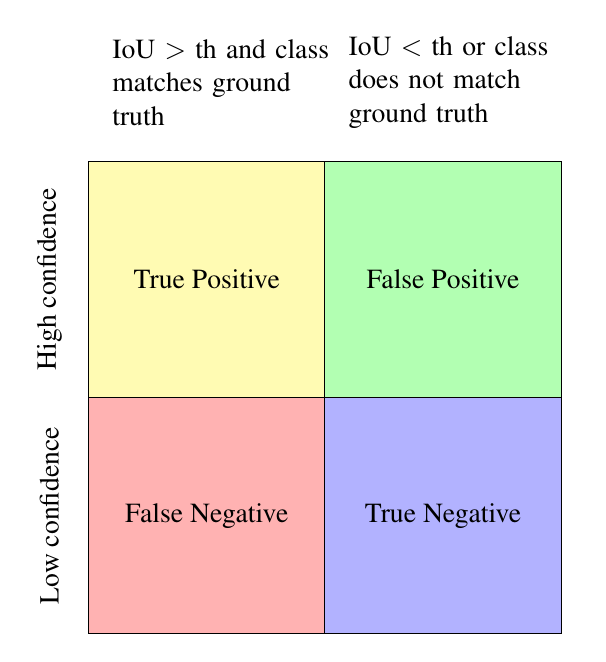
\begin{tikzpicture}
    \draw[draw=black,fill=yellow!30] (0,0) rectangle (3,3);
    \draw[draw=black,fill=green!30] (3,0) rectangle (6,3);
    \draw[draw=black,fill=red!30] (0,-3) rectangle (3,0);
    \draw[draw=black,fill=blue!30] (3,-3) rectangle (6,0);
    
    \node at (1.5,1.5) {True Positive};
    \node at (4.5,1.5) {False Positive};
    \node at (1.5,-1.5) {False Negative};
    \node at (4.5,-1.5) {True Negative};

    \node[text width=2.8cm] at (1.7,4) {IoU \begin{math}>\end{math} th and class matches ground truth};
    \node[text width=2.8cm] at (4.7,4) {IoU \begin{math}<\end{math} th or class does not match ground truth};
    \node[rotate=90] at (-0.5,1.5) {High confidence};
    \node[rotate=90] at (-0.5,-1.5) {Low confidence};
\end{tikzpicture}


\end{document}
	\caption{\label{fig:2_IoU_det} IoU and class match to find the type of detection.}
\end{figure}

\begin{equation}
	\text{IoU} = \frac{\text{area of intersection}}{\text{area of union}}
	\label{eq:IoU}
\end{equation}

Each detection can be put into one of four categories shown in the figure, based on if and how well it matches the ground truth, listed below.

\begin{itemize}
	\item True positive: The model correctly detects an object and the IoU is above the threshold.
	\item False positive: The model detects an object but the IoU is below the threshold or the model mislabels the object.
	\item False negative: The model does not detect an object but it should have.
	\item True negative: The model does not detect an object and it should not have, this is not used in the metrics as it is not very useful.
\end{itemize}

Using this a few key metrics can be calculated. The main metrics we will use are precision, recall and their derivatives. Precision (\ref{eq:precision}) is the ratio of true positives to the total number of positives. Recall (\ref{eq:recall}) is the ratio of true positives to the total number of detectable positives.



\begin{equation}
	Precision = \frac{TruePositives}{True Positives + False Positives}
	\label{eq:precision}
\end{equation}

\begin{equation}
	Recall = \frac{True Positives}{True Positives + False Negatives}
	\label{eq:recall}
\end{equation}

The model assigns each detection a confidence score, the dividing threshold between high and low confidence can be chosen freely. A high confidence threshold will result in a low recall but high precision. A low confidence threshold will result in a high recall but low precision. Plotting the precision and recall against the threshold results in a precision-recall curve.

Averaging the precision across all recall levels results in the average precision (AP) metric. Averaging the AP over all classes results in the mean average precision (mAP) metric. The mAP is the most common metric used to evaluate object detection models.

\section{Conclusion}

\begin{table}[H]
	\begin{tabular}{lll}\cline{2-3}
	\multicolumn{1}{l|}{}                         & \multicolumn{1}{l|}{Scores on COCO} & \multicolumn{1}{l|}{Special characteristic}\\ \hline
	\multicolumn{1}{|l|}{\multirow{3}{*}{OWL-ViT}} & \multicolumn{1}{l|}{41.8* [1 shot]}          & \multicolumn{1}{l|}{\multirow{3}{*}{K-Shot-N-Way without retraining}}\\ \cline{2-2}
	\multicolumn{1}{|l|}{}                         & \multicolumn{1}{l|}{46.8* [10 shot]}          & \multicolumn{1}{l|}{}\\ \cline{2-2}
	\multicolumn{1}{|l|}{}                         & \multicolumn{1}{l|}{/}              & \multicolumn{1}{l|}{}\\ \hline
	\multicolumn{1}{|l|}{\multirow{3}{*}{imTED}}   & \multicolumn{1}{l|}{/}              & \multicolumn{1}{l|}{\multirow{3}{*}{}}\\ \cline{2-2}
	\multicolumn{1}{|l|}{}                         & \multicolumn{1}{l|}{22.5** [10 shot]}           & \multicolumn{1}{l|}{}\\ \cline{2-2}
	\multicolumn{1}{|l|}{}                         & \multicolumn{1}{l|}{30.2** [30 shot]}           & \multicolumn{1}{l|}{}\\ \hline
	\multicolumn{1}{|l|}{\multirow{3}{*}{hANMCL}}  & \multicolumn{1}{l|}{13.4** [1 shot]}           & \multicolumn{1}{l|}{\multirow{3}{*}{\begin{tabular}[c]{@{}l@{}}1-Shot-N-Way without retraining\\ Faster R-CNN based, so less performant hardware required\\ Contrastive-learning suited to divide metric space of our alike shells\end{tabular}}} \\ \cline{2-2}
	\multicolumn{1}{|l|}{}                         & \multicolumn{1}{l|}{22.4** [10 shot]}           & \multicolumn{1}{l|}{}\\ \cline{2-2}
	\multicolumn{1}{|l|}{}                         & \multicolumn{1}{l|}{25.0** [30 shot]}           & \multicolumn{1}{l|}{}\\ \hline
	\multicolumn{3}{l}{*Results for AP50}\\
	\multicolumn{3}{l}{**Results for AP}
	\end{tabular}
\end{table}
In this chapter, we have studied object counting, with a focus on few-shot object detection. We went into more detail regarding the different ways to implement few-shot learning to detect objects. Studying the SOTA methods for few-shot object detection, we found that a wide variety of models, each with different advantages and disadvantages exist. OWL-ViT and hANMCL are capable of few-shot object detection without finetuning/retraining, thus they are a good fit to establish a baseline. In terms of viability, hANMCL is faster R-CNN-based and uses a convolutional backbone, as opposed to OWL-ViT and imTED which use ViT, an attention-based backbone. Both OWL-ViT and hANMCL can be used to initially establish a baseline as they do not require retraining. For our implementation, we will establish a baseline with OWL-ViT.
%%%%%%%%%%%%%%%%%%%%%%%%%%%%%%%%%%%%%%%%%%%%%%%%%%%%%%%%%%%%%%%%%%% 
%                                                                 %
%                            CHAPTER                              %
%                                                                 %
%%%%%%%%%%%%%%%%%%%%%%%%%%%%%%%%%%%%%%%%%%%%%%%%%%%%%%%%%%%%%%%%%%% 
 
\chapter{Implementation}
In this chapter, we will discuss the implementation. We first introduce the general setup, then we discuss the implementation of the model.

% general
%   brambox
%   BBAnnotatedImage
%     functions
%     __init__
% owl-vit
%   scenic
%     jax
%   detection

\section{General setup}
In this section, we will discuss the general setup, which is universal for any implementation. We will discuss the brambox library which we use for evaluating the results. We will also discuss our own class we use for working with the dataset.

\subsection{Brambox}
Brambox \citep{brambox} (Basic Requisites for Algorithms on iMages toolBOX) is a library for working with object detection algorithms and datasets. It offers functionality for handling annotations and detections, as well as evaluating the results. 

Brambox uses pandas' DataFrames for storing data. The io module offers functions for loading and saving annotations or detections. This allows us to save checkpoints between time or compute-intensive steps. We do however have to manually make sure the outputs of our model are put into the correct format. With both annotations and detections in brambox format, the stat module offers functions for evaluating the results like precision-recall (PR) curves and average precision (AP). Plotting these gives us a visual representation of the results.

\subsection{BBAnnotatedImage}
To make working with the dataset easier we made a class that contains both an image and its annotations. Storing these together allows us to change the orientation and scale of our images which we do during initialization, making sure all images are in landscape orientation and optionally resized with a given scale. Besides storing it also offers some functions for working with the image, these can be found in Table \ref{tab:3_bbannotatedimage_functions}. It also makes sure all images are in landscape orientation and optionally resizes them with a given scale during initialization.

\begin{table}[]
    \begin{tabular}{|l|p{3.9cm}|l|p{5cm}|}
    \hline
    Function    & Arguments                                    & Type   & Description                     \\ \hline
    from\_xml() & xml\_filepath, image\_dir, (optional: scale) & Static & Initialize class from xml\_file \\ \hline
    draw\_annotations() & (optional: resize) & & Draw annotations on image and return (optionally resized)\\ \hline
    object\_image\_cutouts() & & Property & Return cutouts of the annotated objects \\ \hline
    objects() & & Property & Return a list of tuples containing cutouts and their class \\ \hline
    npimage() & & Property & Return the image as NumPy array \\ \hline

    \end{tabular}
    \centering
    \caption{Functions of the BBAnnotatedImage class.}
    \label{tab:3_bbannotatedimage_functions}
\end{table}

\section{OWL-ViT}
In this section, we will discuss the implementation of the OWL-ViT model. We will first discuss Scenic, in which OWL-ViT is implemented. Then we will discuss our specific implementation of the model.

\subsection{Scenic}
"Scenic is a codebase with a focus on research around attention-based models for computer vision ... More precisely, Scenic is a: (i) set of shared light-weight libraries solving tasks commonly encountered tasks when training large-scale (i.e. multi-device, multi-host) vision models; and (ii) several projects containing fully fleshed out problem-specific training and evaluation loops using these libraries." as per \citet{scenic}.

The model we will use is one such project that is included in Scenic. When the OWL-ViT model was first introduced, an online "playground" was made available where the model could be tested by anyone. Though it is no longer available, the jupyter notebook used for it is included as part of the OWL-ViT project in Scenic. This notebook is used as the basis for the implementation of the model.

\subsection{Notebook implementation} \label{sec:3_notebook_implementation}
While the notebook does give us a good starting point, we mostly just use the inference module it uses while discarding the rest as it was intended for the visual-only online playground and we're mostly interested in statistics. 

\subsubsection*{Setup}

We start by loading our dataset into a list of BBAnnotatedImages by looping over all XML files in our annotations folder and loading them using the BBAnnotatedImage.from\_xml() function. 

The loading of the model is unchanged, except we use a larger version of the model. The playground used CLIP B16, while we're using CLIP L14. A previous iteration of this paper used CLIP B32.

\subsubsection*{Inference}

We first obtain the embeddings. For text embeddings, this is easy as the inference module has a function that takes a tuple with any amount of strings and returns the embeddings. For image embeddings, only 1-shot 1-way inference was implemented in the playground. We can however implement k-shot by averaging multiple embeddings of the same class. By afterward simply merging these into a single NumPy array, we can use the same function for inference as for text embeddings (model.get\_scores()). To reduce the number of images we have to remove from the test set, we start by calculating embeddings for the class with the least amount of annotations and work our way up. As we remove all images from which we get our query embeddings, we could use all annotations from those images, instead of limiting ourselves to N-shot. Though interesting to do, it goes against the definition of N-shot learning.

Next, we create a DataFrame in the Brambox format at the exact size to store all our detections. We then loop over all images in our dataset, adding the detections to the DataFrame after making sure they are in the correct format (OWL-ViT returns normalized centered coordinates, while Brambox expects absolute top-left coordinates). 

\subsubsection*{Post-processing and evaluation} 

We add an 'IoU' column to the DataFrame, which we fill with the threshold at which the detection will be eliminated when we do non-maximum suppression (NMS). 

We optionally remove the labels from both the annotations and detections, to see how to model performs at detecting objects, regardless of class. 

To evaluate the results, we use Brambox to calculate the PR curves and AP for various IoU thresholds. We also save some images with annotations and detections for various IoU and confidence thresholds for a more visual representation of the results.
%%%%%%%%%%%%%%%%%%%%%%%%%%%%%%%%%%%%%%%%%%%%%%%%%%%%%%%%%%%%%%%%%%% 
%                                                                 %
%                            CHAPTER                              %
%                                                                 %
%%%%%%%%%%%%%%%%%%%%%%%%%%%%%%%%%%%%%%%%%%%%%%%%%%%%%%%%%%%%%%%%%%% 
\chapter{Results}
In this chapter, we will discuss the results of applying the OWL-ViT model to the shell dataset. We will first use the model as a zero-shot object detector. Secondly, we will use it as a N-shot object detector. For both, we will discuss the results for generic shell detection and detecting and classifying the shells. All PR-curve figures can be found in full size in Appendix \ref{app:pr_curves_full_size}.

\section{Zero-shot object detection}
For zero-shot object detection, we use the model with text embeddings. We also tried using negative queries, but this did not improve the results. For classless object detection, we added a few generic descriptions like 'seashell' and 'shell' to the queries.


% image with 2 subimages side by side (a) and (b)
\begin{figure}[h]
    \begin{adjustwidth}{-0.5in}{-0.5in}
        \centering
        \begin{subfigure}[b]{0.38\pdfpagewidth}
            \includegraphics[width=\textwidth]{chapter5/text/classlessIoUPR.png}
            \caption{PR curve classless zero-shot object detection.}
            \label{fig:5_zero_shot_classless}
        \end{subfigure}
        \hfill
        \begin{subfigure}[b]{0.38\pdfpagewidth}
            \includegraphics[width=\textwidth]{chapter5/text/classedIoUPR.png}
            \caption{PR curve classed zero-shot object detection.}
            \label{fig:5_zero_shot_classed}
        \end{subfigure}
    \end{adjustwidth}
    \caption{Zero-shot object detection.}
    \label{fig:5_zero_shot}
\end{figure}

For the classless detection, as seen in Fig \ref{fig:5_zero_shot_classed}, we obtain an AP of 42.26\% and an F1-score of 44.75\%. This seems like it could be used to generate proposals for manual classification. Upon visual inspection, however, we find very inconsistent results across images, as can be seen in Table \ref{fig:5_zero_shot_classless_examples}.

\begin{table}[h]
    % columns: threshold, image1, image2
    \centering
    \captionsetup{justification=centering}
    \begin{tabular}{|l|ll|}
        \hline
        Score & Image 1 & Image 2 \\ \hline
        0.1 & \includegraphics[width=0.4\textwidth]{chapter5/text/classless/0.1/1.jpg} & \includegraphics[width=0.4\textwidth]{chapter5/text/classless/0.1/3.jpg} \\ \hline
        0.2 & \includegraphics[width=0.4\textwidth]{chapter5/text/classless/0.2/1.jpg} & \includegraphics[width=0.4\textwidth]{chapter5/text/classless/0.2/3.jpg} \\ \hline
        0.3 & \includegraphics[width=0.4\textwidth]{chapter5/text/classless/0.3/1.jpg} & \includegraphics[width=0.4\textwidth]{chapter5/text/classless/0.3/3.jpg} \\ \hline
    \end{tabular}
    \caption{Examples of classless zero-shot object detection.}
    \label{fig:5_zero_shot_classless_examples}
\end{table}

For normal object detection, however, results aren't that great, with an mAP of 1.83\% and an F1-score of 10.71\%. When we look at the PR-curve for individual classes in Fig \ref{fig:5_zero_shot_classed_classes_PR} we find that some classes aren't even found at all.

\begin{figure}[h]
    \centering
    \includegraphics[width=0.7\textwidth]{chapter5/text/classesPR.png}
    \caption{PR curve for individual classes in zero-shot object detection.}
    \label{fig:5_zero_shot_classed_classes_PR}
\end{figure}

\section{N-shot object detection}
For N-shot object detection, we use the model with image embeddings. As the model now has visual examples of our objects, we expect better results than with zero-shot object detection. We will start by testing one-shot object detection, then we will test N-shot object detection with different values for N.

\subsection*{One-shot object detection}
One-shot object detection has always been quite a challenge, as it is difficult to learn a good representation of an object with only one example. As OWL-ViT is the SOTA model for this task, with some room to spare, we expect it to perform better than our zero-shot object detection. 

\begin{figure}[h]
    \begin{adjustwidth}{-0.5in}{-0.5in}
        \centering
        \begin{subfigure}[b]{0.4\pdfpagewidth}
            \includegraphics[width=\textwidth]{chapter5/img/classless\_1\_iouPR.png}
            \caption{PR curve classless.}
            \label{fig:5_n_shot_classless_pr_curve}
        \end{subfigure}
        \hfill
        \begin{subfigure}[b]{0.4\pdfpagewidth}
            \includegraphics[width=\textwidth]{chapter5/img/classed\_1\_iouPR.png}
            \caption{PR curve with classes.}
            \label{fig:5_n_shot_classed}
        \end{subfigure}
    \end{adjustwidth}
    \caption{1-shot object detection.}
    \label{fig:5_1_shot}
\end{figure}

For classless object detection, as seen in Fig \ref{fig:5_1_shot}, we obtain an AP of 40.89\% and an F1-score of 43.68\%. This is slightly worse than our zero-shot object detection. Upon visual inspection, we find that the model is more consistent in its detections, but still marks too many shards or parts of shells as detections, as can be seen in Table \ref{fig:5_n_shot_classless_examples}.

\begin{table}[H]
    % columns: threshold, image1, image2
    \centering
    \captionsetup{justification=centering}
    \begin{tabular}{|l|ll|}
        \hline
        Score & Image 1 & Image 2 \\ \hline
        0.7 & \includegraphics[width=0.35\textwidth]{chapter5/img/1_classless/0.7/1.jpg} & \includegraphics[width=0.35\textwidth]{chapter5/img/1_classless/0.7/2.jpg} \\ \hline
        0.8 & \includegraphics[width=0.35\textwidth]{chapter5/img/1_classless/0.8/1.jpg} & \includegraphics[width=0.35\textwidth]{chapter5/img/1_classless/0.8/2.jpg} \\ \hline
        0.9 & \includegraphics[width=0.35\textwidth]{chapter5/img/1_classless/0.9/1.jpg} & \includegraphics[width=0.35\textwidth]{chapter5/img/1_classless/0.9/2.jpg} \\ \hline
    \end{tabular}
    \caption{Examples of classless 1-shot object detection.}
    \label{fig:5_n_shot_classless_examples}
\end{table}

For normal object detection, however, results are better than with 0-shot, with an mAP of 5.46\% and an F1-score of 15.54\%. While this is still not great or useable, it is a significant improvement over 0-shot. When we look at the PR-curve for individual classes in Fig \ref{fig:5_n_shot_classed_classes_PR} we find a general improvement across the board.

\begin{figure}[H]
    \centering
    \includegraphics[width=0.7\textwidth]{chapter5/img/classed_1_classesPR.png}
    \caption{PR curve for individual classes in 1-shot object detection.}
    \label{fig:5_1_shot_classed_classes_PR}
\end{figure}

\subsection*{N-shot object detection}
Extracting multiple image embeddings and averaging those allows us to obtain more robust embeddings. This should reduce false detections and allow the model to better identify shells in difficult positions, like mostly buried or flipped shells. We will test this by using different values for N and comparing the results. The results can be found in Table \ref{tab:5_n_shot_results}. The PR curves for all N can be found in Appendix \ref{app:pr_curves_n_shot}. A visual comparison can be found in Table \ref{fig:5_n_shot_examples}.

\begin{table}[H]
    \centering
    \captionsetup{justification=centering}
    \begin{tabular}{|l|l|l|}
        \hline
        N & Classless AP & Classed mAP \\ \hline
        5 & 45.91 & 7.01 \\ \hline
        10 & 55.88 & 15.37 \\ \hline
        20 & 48.40 & 13.55 \\ \hline
        50 & 42.91 & 30.17 \\ \hline
    \end{tabular}
    \caption{Results for N-shot object detection.}
    \label{tab:5_n_shot_results}
\end{table}


\begin{table}[H]
    \begin{adjustwidth}{-0.5in}{-0.5in}
        % columns: N, image1, image2
        \centering
        \captionsetup{justification=centering}
        \begin{tabular}{|l|ll|}
            \hline
            N & Image 1 & Image 2 \\ \hline
            5 & \includegraphics[width=0.4\pdfpagewidth]{chapter5/img/5_classed/IMG20230217103106.jpg} & \includegraphics[width=0.4\pdfpagewidth]{chapter5/img/5_classed/IMG20230217104210.jpg} \\ \hline
            10 & \includegraphics[width=0.4\pdfpagewidth]{chapter5/img/10_classed/IMG20230217103106.jpg} & \includegraphics[width=0.4\pdfpagewidth]{chapter5/img/10_classed/IMG20230217104210.jpg} \\ \hline
            20 & \includegraphics[width=0.4\pdfpagewidth]{chapter5/img/20_classed/IMG20230217103106.jpg} & \includegraphics[width=0.4\pdfpagewidth]{chapter5/img/20_classed/IMG20230217104210.jpg} \\ \hline
        \end{tabular}
        \caption{Examples of classed N-shot object detection.}
        \label{fig:5_n_shot_examples}
    \end{adjustwidth}
\end{table}


We find a large peak in performance for 50-shot, important to consider though is that classes with fewer annotations than N are discarded. Looking at Fig \ref{fig:5_50_shot_classed_classes_PR} we see that we're only evaluating 4 classes. These classes also have the most unique features, which makes them easier to detect. The 50-shot results are thus not representative and should be discarded.

\begin{figure}[H]
    \centering
    \begin{adjustwidth}{-0.5in}{-0.5in}
        \begin{subfigure}[b]{0.4\pdfpagewidth}
            \includegraphics[width=\textwidth]{chapter5/img/classed_5_classesPR.png}
            \caption{PR curves for 5-shot object detection.}
            \label{fig:5_5_shot_classed_classes_PR}
        \end{subfigure}
        \hfill
        \begin{subfigure}[b]{0.4\pdfpagewidth}
            \includegraphics[width=\textwidth]{chapter5/img/classed_10_classesPR.png}
            \caption{PR curves for 10-shot object detection.}
            \label{fig:5_10_shot_classed_classes_PR}
        \end{subfigure}
        \begin{subfigure}[b]{0.4\pdfpagewidth}
            \includegraphics[width=\textwidth]{chapter5/img/classed_20_classesPR.png}
            \caption{PR curves for 20-shot object detection.}
            \label{fig:5_20_shot_classed_classes_PR}
        \end{subfigure}
        \hfill
        \begin{subfigure}[b]{0.4\pdfpagewidth}
            \includegraphics[width=\textwidth]{chapter5/img/classed_50_classesPR.png}
            \caption{PR curves for 50-shot object detection.}
            \label{fig:5_50_shot_classed_classes_PR}
        \end{subfigure}
        \caption{PR curves for individual classes in N-shot object detection.}
        \label{fig:5_n_shot_classed_classes_PR}
    \end{adjustwidth}
\end{figure}

\section{Using all embeddings}
As mentioned before in Section \ref{sec:3_notebook_implementation} we currently throw away a lot of generated embeddings as they go over the N-amount of N-shot. Using these could on the other hand be compared to a train-test split (no validation set is required as we're not training). For our most common type of shells, this could bring a major improvement to the robustness of the embeddings. The results for this can be found in Table \ref{tab:5_all_embeddings_results}, here N is the minimum number of embeddings for a class instead of an exact amount of embeddings per class. The highest impact is, as expected since the base robustness is lower, on the lower values for N. For certain options, we do see a slight degradation in performance, but overall the results are slightly better than with the exact N-shot.

\begin{table}[H]
    \centering
    \captionsetup{justification=centering}
    \begin{tabular}{|l|l|l|}
        \hline
        N & Classless AP (strict N) & Classed mAP (strict N) \\ \hline
        1 & 55.05 (40.89) & 14.61 (5.46) \\ \hline
        5 & 56.18 (45.91) & 13.36 (7.01) \\ \hline
        10 & 57.90 (55.88) & 14.30 (15.37) \\ \hline
        20 & 51.45 (48.40) & 17.20 (13.55) \\ \hline
        50 & 42.45 (42.91) & 27.83 (30.17) \\ \hline
    \end{tabular}
    \caption{Results for N-shot object detection using all embeddings.}
    \label{tab:5_all_embeddings_results}
\end{table}

\section{Discussion}
Visually inspecting our results we find some reasons for the mediocre results, like false positives and wrong detections.

\subsection*{False positives}
The model finds many shells in places without annotations. These detections range from rocks to unidentifiable fragments to broken shells to shells we missed during annotating. Most false positives at high confidence are of the last two types. Solving this would have little to do with our implementation, but rather with the dataset. Annotating the dataset better is easier said than done, as not every shell is easy to annotate. We will go into more detail on this in the next section.

\subsection*{Dataset quality}
Annotating the shell dataset isn't easy. We are not experts who can see the minute details that differentiate two similar shells, like the 'cut trough shell' and the 'thick trough shell' as shown in Fig \ref{fig:5_wikipedia_cut_vs_thick}. We also have to deal with shells that are mostly buried or broken, how broken should a shell be but still be annotated? Some shells, like the cockle, have a very recognizable pattern even in fragments. Expanding the dataset would also possibly make other methods possible besides few-shot object detection or it would at least give us more robust results.


\begin{figure}[H]
    \centering
    \begin{subfigure}[b]{\textwidth}
        \includegraphics[width=\textwidth]{chapter5/wikipedia\_cut\_trough\_shell\_small.jpg}
        \caption{The cut trough shell.}
        \label{fig:5_wikipedia_cut_trough_shell}
    \end{subfigure}
    \hfill
    \begin{subfigure}[b]{\textwidth}
        \includegraphics[width=\textwidth]{chapter5/wikipedia\_thick\_trough\_shell\_small.jpg}
        \caption{The thick trough shell.}
        \label{fig:5_wikipedia_thick_trough_shell}
    \end{subfigure}
    \caption{The cut trough shell and the thick trough shell. Images from Wikipedia.}
    \label{fig:5_wikipedia_cut_vs_thick}
\end{figure}


%%%%%%%%%%%%%%%%%%%%%%%%%%%%%%%%%%%%%%%%%%%%%%%%%%%%%%%%%%%%%%%%%%% 
%                                                                 %
%                            CHAPTER                              %
%                                                                 %
%%%%%%%%%%%%%%%%%%%%%%%%%%%%%%%%%%%%%%%%%%%%%%%%%%%%%%%%%%%%%%%%%%% 
\chapter{Conclusion}

In this thesis, we applied object detection to the field of shell detection. We created a small dataset of seashells as no such dataset existed. As the dataset is too small to apply traditional object detection, we used zero- and few-shot object detection using the OWL-ViT model.

We found that zero-shot object detection is not performant enough to be used for shell detection, we suspect that this is due to the specific shell names never having been given during training. This is confirmed by trying classless object detection, with more generic keywords like 'shell' or 'seashell' as this yields better results. This classless detection seemed like it could be used to generate bounding box proposals for manual classification, however, we found that the results were too inconsistent to be used for this.

We then explored few-shot object detection with various values for N. We found that for certain shells with distinct features, the model was able to detect them with a high accuracy. However, for shells that are more similar to each other, the model was not able to differentiate between them. This was to be expected as a human also has difficulty differentiating between these shells. The model could be used to detect certain shells with a high accuracy, but it is not able to detect all shells reliably. This is especially an issue if we want to use the model to detect shells that are currently not present in the dataset as some of those shells will be very similar to one another too.

In conclusion, we found that the current SOTA in few-shot object detection could be used as an assisting tool for shell detection, but it is not able to reliably work independently. 


\section*{Future work}
In this section, we will discuss some possible future work that could be done to improve the results of this thesis.

\begin{itemize}
    \item Expand the dataset with more images and annotations: The current dataset is quite limited in size and variety. If more interest is shown in this field, it would be possible to further expand the dataset. This would open more avenues for future work, such as using more data-intensive trained models like YOLO or Faster R-CNN.
    \item Correct the dataset: The dataset contains some annotations that are not correct. This causes the model to be wrongly punished at times. This is due to us not being experts in the field of seashells. By working more closely with experts, it would be possible to correct these annotations.
\end{itemize}
% Bibliografie: referenties. De items zitten in bibliografie.bib
%%%%%%%%%%%%%%%%%%%%%%%%%%%%%%%%%%%%%%%%%%%%%%%%%%%%%%%%%%%%%%%%%
% Indien je ook de niet geciteerde werken in je bibliografie wil opnemen, commentarieer dan onderstaande regel uit!
%\nocite{*}
\bibliographystyle{plainnat}
\bibliography{bibliografie}

% Eventueel enkele appendices
%%%%%%%%%%%%%%%%%%%%%%%%%%%%%%
\appendix
\chapter{PR curves at full size} \label{app:pr_curves_full_size}


\begin{figure}[H]
    \includegraphics[width=\textwidth]{chapter5/text/classlessIoUPR.png}
    \caption{PR curve classless zero-shot object detection.}
    \label{fig:zero_shot_classless_appendix}
\end{figure}

\begin{figure}[H]
    \includegraphics[width=\textwidth]{chapter5/text/classedIoUPR.png}
    \caption{PR curve classed zero-shot object detection.}
    \label{fig:zero_shot_classed_appendix}
\end{figure}

\begin{figure}[H]
    \includegraphics[width=\textwidth]{chapter5/text/classesPR.png}
    \caption{PR curve individual classes in zero-shot object detection.}
    \label{fig:zero_shot_classed_classes_PR_appendix}
\end{figure}

\begin{figure}[H]
    \includegraphics[width=\textwidth]{chapter5/img/classless\_1\_iouPR.png}
    \caption{PR curve classless 1-shot object detection.}
    \label{fig:1_shot_appendix}
\end{figure}

\begin{figure}[H]
    \includegraphics[width=\textwidth]{chapter5/img/classed\_1\_iouPR.png}
    \caption{PR curve classed 1-shot object detection.}
    \label{fig:2_shot_appendix}
\end{figure}




\chapter{PR curves for N shot} \label{app:pr_curves_n_shot}

\begin{figure}[H]
    \begin{adjustwidth}{-0.5in}{-0.5in}
        \centering
        \begin{subfigure}[b]{0.4\pdfpagewidth}
            \includegraphics[width=\textwidth]{chapter5/img/classless\_5\_iouPR.png}
            \caption{PR curve 5-shot object detection.}
            \label{fig:5_n_shot_classless_5}
        \end{subfigure}
        \hfill
        \begin{subfigure}[b]{0.4\pdfpagewidth}
            \includegraphics[width=\textwidth]{chapter5/img/classless\_10\_iouPR.png}
            \caption{PR curve 10-shot object detection.}
            \label{fig:5_n_shot_classless_10}
        \end{subfigure}
        \begin{subfigure}[b]{0.4\pdfpagewidth}
            \includegraphics[width=\textwidth]{chapter5/img/classless\_20\_iouPR.png}
            \caption{PR curve 20-shot object detection.}
            \label{fig:5_n_shot_classless_20}
        \end{subfigure}
        \hfill
        \begin{subfigure}[b]{0.4\pdfpagewidth}
            \includegraphics[width=\textwidth]{chapter5/img/classless\_50\_iouPR.png}
            \caption{PR curve 50-shot object detection.}
            \label{fig:5_n_shot_classless_50}
        \end{subfigure}
    \end{adjustwidth}
    \caption{N-shot classless object detection.}
    \label{fig:5_n_shot_classless}
\end{figure}


\begin{figure}[H]
    \begin{adjustwidth}{-0.5in}{-0.5in}
        \centering
        \begin{subfigure}[b]{0.4\pdfpagewidth}
            \includegraphics[width=\textwidth]{chapter5/img/classed\_5\_iouPR.png}
            \caption{PR curve 5-shot object detection.}
            \label{fig:5_n_shot_classed_5}
        \end{subfigure}
        \hfill
        \begin{subfigure}[b]{0.4\pdfpagewidth}
            \includegraphics[width=\textwidth]{chapter5/img/classed\_10\_iouPR.png}
            \caption{PR curve 10-shot object detection.}
            \label{fig:5_n_shot_classed_10}
        \end{subfigure}
        \begin{subfigure}[b]{0.4\pdfpagewidth}
            \includegraphics[width=\textwidth]{chapter5/img/classed\_20\_iouPR.png}
            \caption{PR curve 20-shot object detection.}
            \label{fig:5_n_shot_classed_20}
        \end{subfigure}
        \hfill
        \begin{subfigure}[b]{0.4\pdfpagewidth}
            \includegraphics[width=\textwidth]{chapter5/img/classed\_50\_iouPR.png}
            \caption{PR curve 50-shot object detection.}
            \label{fig:5_n_shot_classed_50}
        \end{subfigure}
    \end{adjustwidth}
    \caption{N-shot object detection.}
    \label{fig:5_n_shot}
\end{figure}

% Back cover: change according to the correct campus
%\includepdf{private/back_fiiw_denayer.pdf}
\includepdf{private/back_fiiw_denayer_eng.pdf} % For the English version
%\includepdf{private/back_fiiw_geel.pdf}
% \includepdf{private/back_fiiw_geel_eng.pdf} % For the English version
%\includepdf{private/back_fiiw_gent.pdf}
% \includepdf{private/back_fiiw_ghent_eng.pdf} % For the English version
%\includepdf{private/back_fiiw_brugge.pdf}
% \includepdf{private/back_fiiw_bruges_eng.pdf} % For the English version
%\includepdf{private/back_fiiw_groept.pdf}
% \includepdf{private/back_fiiw_groupt_eng.pdf} % For the English version

\end{document}
